\def\figh{2in}
\def\bfigh{2in}
\appendtographicspath{{media/}}

\section{Introduction}
We are interested in obtaining agents that perform optimally on a task involving
uncertainty while being as “simple” as possible, as measured by the size of their
internal “representation”. While this is a problem relevant in many fields, our
motivation comes from the fields of robotics and computer vision. Embodied
agents have sensors providing very high-dimensional data; the world’s state is
similarly high dimensional. Representing the agent’s belief about the world is
complicated enough, and often inference is intractable. However, it has been
observed that, for certain tasks, it is not necessary to represent and plan using the
entire belief.
Therefore, it is interesting to understand whether it is possible to solve a
planning problem using a smaller representation than the entire belief. We will
show that it is indeed possible and we will provide a constructive algorithm to
obtain “representation-minimal” agents.
\begin{figure}
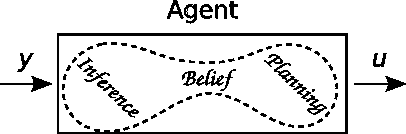
\includegraphics[height=0.7in]{agent}\qquad
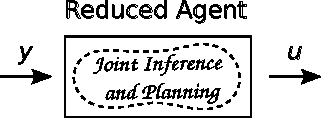
\includegraphics[height=0.7in]{reduced_agent}
\caption{\emph{Representation Reduction} Canonical belief spaces can become a serious informational bottleneck
between inference and planning modules.  
An agent's understanding of its environment need not be any richer than necessary
to support the task at hand.}
\end{figure}
\subsection{Previous Work}
The topic of reduction of logical functions has been extensively studied.
The formalism of finite state machines was developed in the 1950s and 60s,
and by 1971, Hopcroft \cite{hopcroft1971n} published an $(n\log n)$-time algorithm for 
reducing completely-specified FSMs. 
Incompletely-Specified FSMs were studied in turn, and various heuristics were 
developed to quickly approximate minimum\footnote{Here, we distinguish ``minimal'' from ``minimum'' reductions.  
A minimal reduction is one that cannot be further reduced by combining any of its states, whereas
a minimum reduction is a minimal reduction with the fewest possible states} 
 reductions. \cite{Pfleeger:1973:SRI:1311965.1312829,grasselli1965method,goren2007state}.
 Representation reduction in artificial intelligence has been dealt with in various guises:
 Dimensionality reduction, belief space compression etc.\ -- most heuristics can be considered as
 implicit hard-coded representation reductions.
\subsection{Contributions}
This chapter re-casts problem of representation reduction in terms of well-studied computational constructs,
and finds absolute minimum reductions in the case of discrete time, discrete input and output.
It evaluates three algorithms for approximating minimum reductions, and clarifies their strengths and weaknesses.
This work is the result of a collaboration of Andrea Censi, 
who introduced the formalism of representation reduction in the context of POMDP solvers
and proposed the bit-at-a-time algorithm
\section{Formalization}
\iffalse
\begin{definition}[Finite State Machine]
 A finite state machine is a tuple
 $$\ang{\Sigma, \Gamma, S, S_0, \delta, \omega},$$
 where $\Sigma$ and $\Gamma$ are finite input and ouput alphabets, $S$ is a finite set of states, $s_0\in S$ is an initial state,
 $\delta:S\times\Sigma\to S$ is a state-transition function, and $\omega:S\times\Sigma\to\Gamma$ is an output function.
\end{definition}
This generalizes to
\begin{definition}[Incompletely-Specified Finite State Machine (ISFSM)]
 An incompletely-specified finite state machine is a tuple
$$\ang{\Sigma, \Gamma, S, s_0 , \delta, \omega},$$
where $\Sigma$ and $\Gamma$ are finite input and ouput alphabets, $S$ is a finite set of states, $s_0\in S$ is an initial state,
 $\delta:S\times\Sigma\to S\cup\{\phi\}$ is a state-transition function, and $\omega:S\times\Sigma\to\Gamma\cup\{\epsilon\}$ is an output function.
The extra symbols $\phi\notin S$ and $\epsilon\notin\Gamma$ denote ``unspecified'' outputs, 
whose associated input and state are not expected to occur.
s\end{definition}
\begin{definition}[Policy]
 A decision policy is a tuple
 $\ang{\C,\U,T,\Y}$, where $\U$ is a set of actions, $\Y$ is a set of observations, $\C$ is a set of ``contexts'', (usually taken as the set of finite sequences in $\Y$), and
 and $T:(\C\times\Y)\to \U\cup\{\epsilon\}$ is a ``decision table'', assigning an action to each possible observation, for each context $c\in\C$.  
 Again $\epsilon$ is assigned to unexpected combinations of observation and context.
\end{definition}
\begin{definition}[Obedience]
Given the decision policy $P = \ang{\U, T : \operatorname{Sequences}(\Y)\to\U\cup\{\epsilon\}}$, we say
that an ISFSM $\ang{\Sigma, \Gamma, S, s_0, \delta, \omega}$ obeys the policy $P$ if for every finite
sequence $y_1, \ldots, y_n \in \Y$, there exists a sequence $s_0, \ldots, s_{n−1} \subs S$ such that
$s_i = \delta(s_{i−1} , y_i)$ for all $i = 1, \ldots, n$
and
$T(y_1, \ldots, y_n ) = \omega(s_{n−1} , y_n$
or
$T (y_1 , ... , y_n ) = \epsilon$.
\end{definition}


\begin{example}[Equivalent Decision Tables] \label{ex:complete}
Suppose $\Y=\{1,2\}$, $\U=\{A,B\}$, $\C=\bigcup_{i=1}^2\Y^i$ and 
$$\T(c) = \begin{cases}
A & c \in \{(1), (1,2)\}\\
B & c \in \{(2), (2,1)\}\\
\tT(c) & \text{otherwise.}
\end{cases},$$
is an optimal policy, for arbitrary $\tT:\C\to\U$. However, depending on the choice of $\tT$ (highlighted in the tables below),
the completed policy can have differently-sized minimal representations:

\begin{figure}[h]
\begin{floatrow}
\subfigure[Decision Table]{
\ffigbox[\FBwidth]{
\begin{tabular}{ll}
\rlap{$\T:\C\to\U$}\\
\hline
$(1)$&$\mapsto A$\\
$(2)$&$\mapsto B$\\
\rowcolor{Gray}
$(1,1)$&$\mapsto A$\\
$(1,2)$&$\mapsto A$\\
$(2,1)$&$\mapsto B$\\
\rowcolor{Gray}
$(2,2)$&$\mapsto B$
\end{tabular}
}{}}\quad
\subfigure[Decision Tree]{
\ffigbox[\FBwidth]{
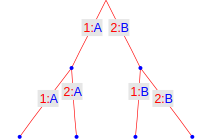
\includegraphics[scale=\sscale]{media/overcomplete_decision}
}{}}\quad\quad
\subfigure[Minimal Policy]{
\ffigbox[\FBwidth]{
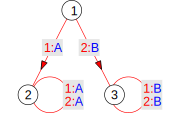
\includegraphics[scale=\sscale]{media/overcomplete-2}
}{}}
\end{floatrow}
\bigskip

\begin{floatrow}
\subfigure[Decision Table]{
\ffigbox[\FBwidth]{
\begin{tabular}{ll}
\rlap{$\T:\C\to\U$}\\
\hline
$(1)$&$\mapsto A$\\
$(2)$&$\mapsto B$\\
\rowcolor{Gray}
$(1,1)$&$\mapsto B$\\
$(1,2)$&$\mapsto A$\\
$(2,1)$&$\mapsto B$\\
\rowcolor{Gray}
$(2,2)$&$\mapsto A$
\end{tabular}
}{}}\quad
\subfigure[Decision Tree]{
\ffigbox[\FBwidth]{
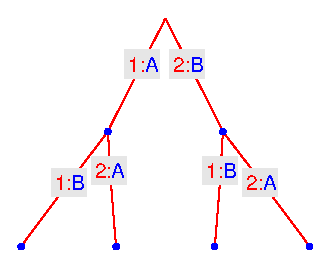
\includegraphics[scale=\sscale]{media/complete_decision}
}{}}\quad\quad
\subfigure[Minimal Policy]{
\hspace{.2cm}
\ffigbox[\FBwidth]{
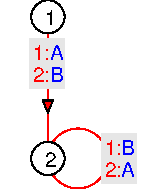
\includegraphics[scale=\sscale]{media/complete-2}
\setcounter{figure}{\value{example}}
\label{fig:best_completion}
}{}}
\end{floatrow}
\end{figure}
\end{example}
Instead, we propose an ``incompletely-determined'' formalization:
\fi
\begin{definition}[Policies]
Given a set $\Y$ of observations, recursively construct
\begin{equation}
\C_0 = \{\emptyset\}\qtx{and}\C_{i+1} = \{(c,y_{i+1})\,:\,c\in\C_i,\, y_{i+1}\in\Y_c\},
\end{equation}
where $\Y_c\subseteq\Y$ are the observations that may be seen in context $c$.  
Let $\C = \bigcup_{i=0}^{\infty}\C_i$.
A \textbf{policy} $P$ is then a tuple $\ang{\C, \U, \T, \Y}$, 
where $\U$ is some decision set and $\T:\C\andn\{\emptyset\}\to\U$.
\end{definition}
\begin{definition}[Completely-Determined Policies]
If $\Y=\bigcup_\C\Y_c$ and $\C=\Y^{\leq n}$ for some $n\in\NN$, then $P=\ang{\C,\U,\T,\Y}$ is \textbf{completely determined}.
A \textbf{completion} of $P$ is a policy $P\1=\ang{\C\1, \U\1, \T\1, \Y}$ such that
\begin{equation}
\Y\subseteq\Y\1,\quad \C\1=\bigcup_{i=0}^{\infty}(\Y\1)^i,\quad \U\subseteq\U\1, \qtx{and} \T\1|_{\C} = \T.
\end{equation}
Let $\Comp(P)$ be the set of completions of the policy $P$.
\end{definition}
\begin{definition}[FSM Representations]
An \textbf{FSM representation} (or just \textbf{representation})
is a tuple $\ang{\C,\R,\U,\S,\T,\Y}$ (abbreviated to $\ang{\R,\S}$ when $P=\ang{\C,\U,\T,\Y}$ is given), 
with ``states'' $\S\subseteq\NN$ and state assignments $\R:\C\to\S$, such that 
\begin{equation}
\R(c)=\R(c\1)\qtx{and}y\in\Y_c\cap\Y_{c\1}\implies\T(c,y)=\T(c\1,y).
\end{equation} 
Let $\Rep(P)$ be the set of representations of the policy $P$.  
\end{definition}
\begin{definition}[Minimal Representations]
The \textbf{size} of an FSM representation is the cardinality of its state set.  
A representation $\ang{\R,\S}$ of $P$ is \textbf{minimal} if 
$|\S|=\min\{|\S\1|\,:\,\ang{\R\1,\S\1}\in\Rep(P)\}$.
A representation $\ang{\R\1,\S\1}$ is a \textbf{reduction} of the representation $\ang{\R,\S}$ if there is a surjection $\phi:\S\to\S\1$
such that $\R\1 = \phi(\R)$.
\end{definition}
\begin{example}
\label{ex:canon}
If $\C = \{c_1, c_2, \ldots\}$, then 
%for any policy $P=\ang{\C,\U,\T,\Y}$,
we have a canonical representation $\ang{\R,\S}$, where
\begin{equation}
\S=\{1,\ldots,|\C|\}\qtx{and}\R:c_k\mapsto k.
\end{equation} 
\end{example}
It can be shown that the size of a minimal representation of a policy $P$ is equal to the minimum
size of the minimal representations of its completions, i.e.
\begin{align}
\min\{|\S\1|\,:\,\ang{\R\1,\S\1}\in\Rep(P)\} = \min\{|\S\1|\,:\,\ang{\R\1,\S\1}\in\Rep(P\1),\,P\1\in\Comp(P)\}
\end{align}
Incompletely-determined policies allow more freedom in representation reduction, as shown in the next example.

\begin{example}[Incompletely-Determined Policies]
Let $\C=\{\emptyset, (1), (2), (1,2), (2,1)\}$, $\U=\{A,B\}$, and
\begin{equation*}
\T(c,y) = \begin{cases}
A & c\in\{(1), (1,2)\}\\
B & c\in\{(2), (2,1)\}
\end{cases}.
\end{equation*}
Observe that the minimal policy is the same as that of the completely-determined policy in Example \ref{fig:best_completion}.
\setcounter{subfigure}{0}
\begin{figure}[h]
\begin{floatrow}
\subfigure[Decision Table]{
\ffigbox[\FBwidth]{
\begin{tabular}{ll}
\multicolumn{2}{c}{$\T:\C\andn\{\emptyset\}\to\U$}\\
\hline
$(1)$&$\mapsto A$\\
$(2)$&$\mapsto B$\\
$(1,2)$&$\mapsto A$\\
$(2,1)$&$\mapsto B$\\
\end{tabular}
}{}}
\subfigure[Decision Tree]{
\ffigbox[\FBwidth]{
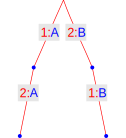
\includegraphics[scale=\sscale]{media/simple_decision}
}{}}\qquad
\subfigure[Representation]{
\ffigbox[\FBwidth]{
\begin{tabular}{ll}
\rlap{$\R:\C\to\S$}\\
\hline
$\emptyset$&$\mapsto 1$\\
$(1)$&$\mapsto 2$\\
$(2)$&$\mapsto 2$\\
$(1,2)$&$\mapsto 2$\\
$(2,1)$&$\mapsto 2$\\
\end{tabular}
}{}}
\subfigure[Minimal Policy]{
\ffigbox[\FBwidth]{
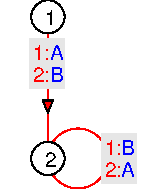
\includegraphics[scale=\sscale]{media/complete-2}
}{}}
\end{floatrow}
\setcounter{figure}{\value{example}}
\label{fig:incomplete}
\end{figure}
\end{example}
\subsection{FSM Reduction}
Given a decision policy (or an ISFSM) how do we find an obedient (or
equivalent) ISFSM with the smallest possible state set?

for completely-specified FSM, this can be done in $n\log n$ time
by Hopcroft's algorithm (Alg.\ \ref{algo: Hopcroft}).


To find a minimum representation of a given policy,
we first compute a graph of reducibility relations, 
then compute a minimal clique-covering.

Cliques on the equivalence graph identify sets of states that can be
collapsed into a single state. The minimal clique-covering, that is the
smallest collection of disjoint cliques that covers the equivalence
graph, correponds to a minimal reduction of the FSM.

\section{Representation Reduction Strategies}


\setcounter{subfigure}{0}
\begin{figure}[ht]
\centering
\subfigure[Canonical Representation]{
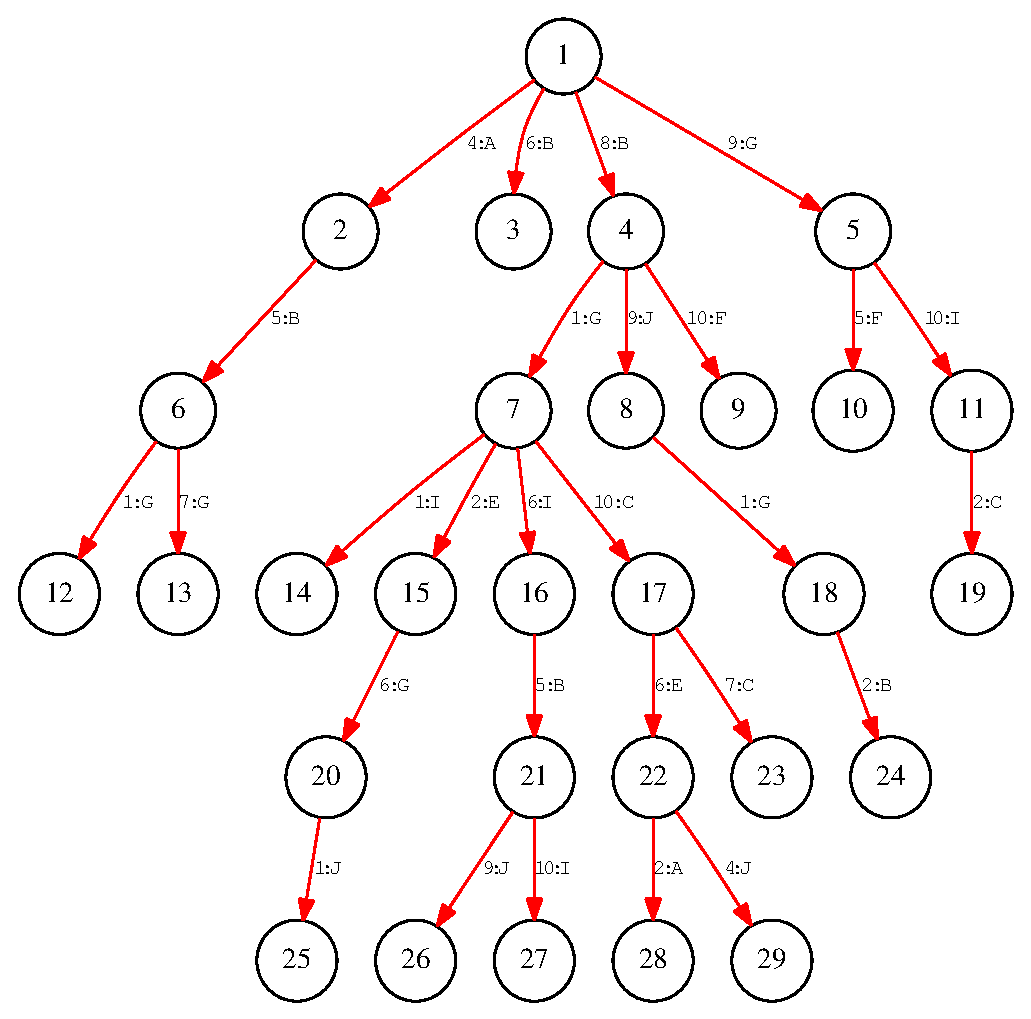
\includegraphics[height=\bfigh]{media/random_alg-1}}\qquad
\subfigure[Compatibility Matrix]{\label{fig:cgam}
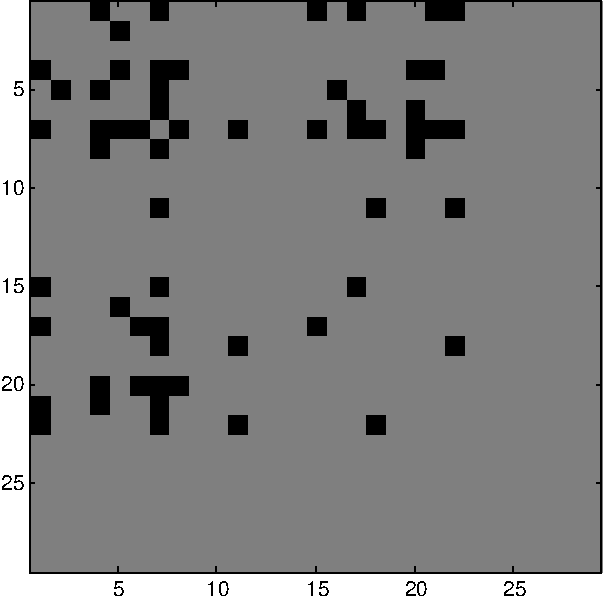
\includegraphics[height=\bfigh]{media/random_adj}}
\end{figure}

\begin{figure}[ht]
\subfigure[Greedy Clique Covering of \ref{fig:cgam}]{
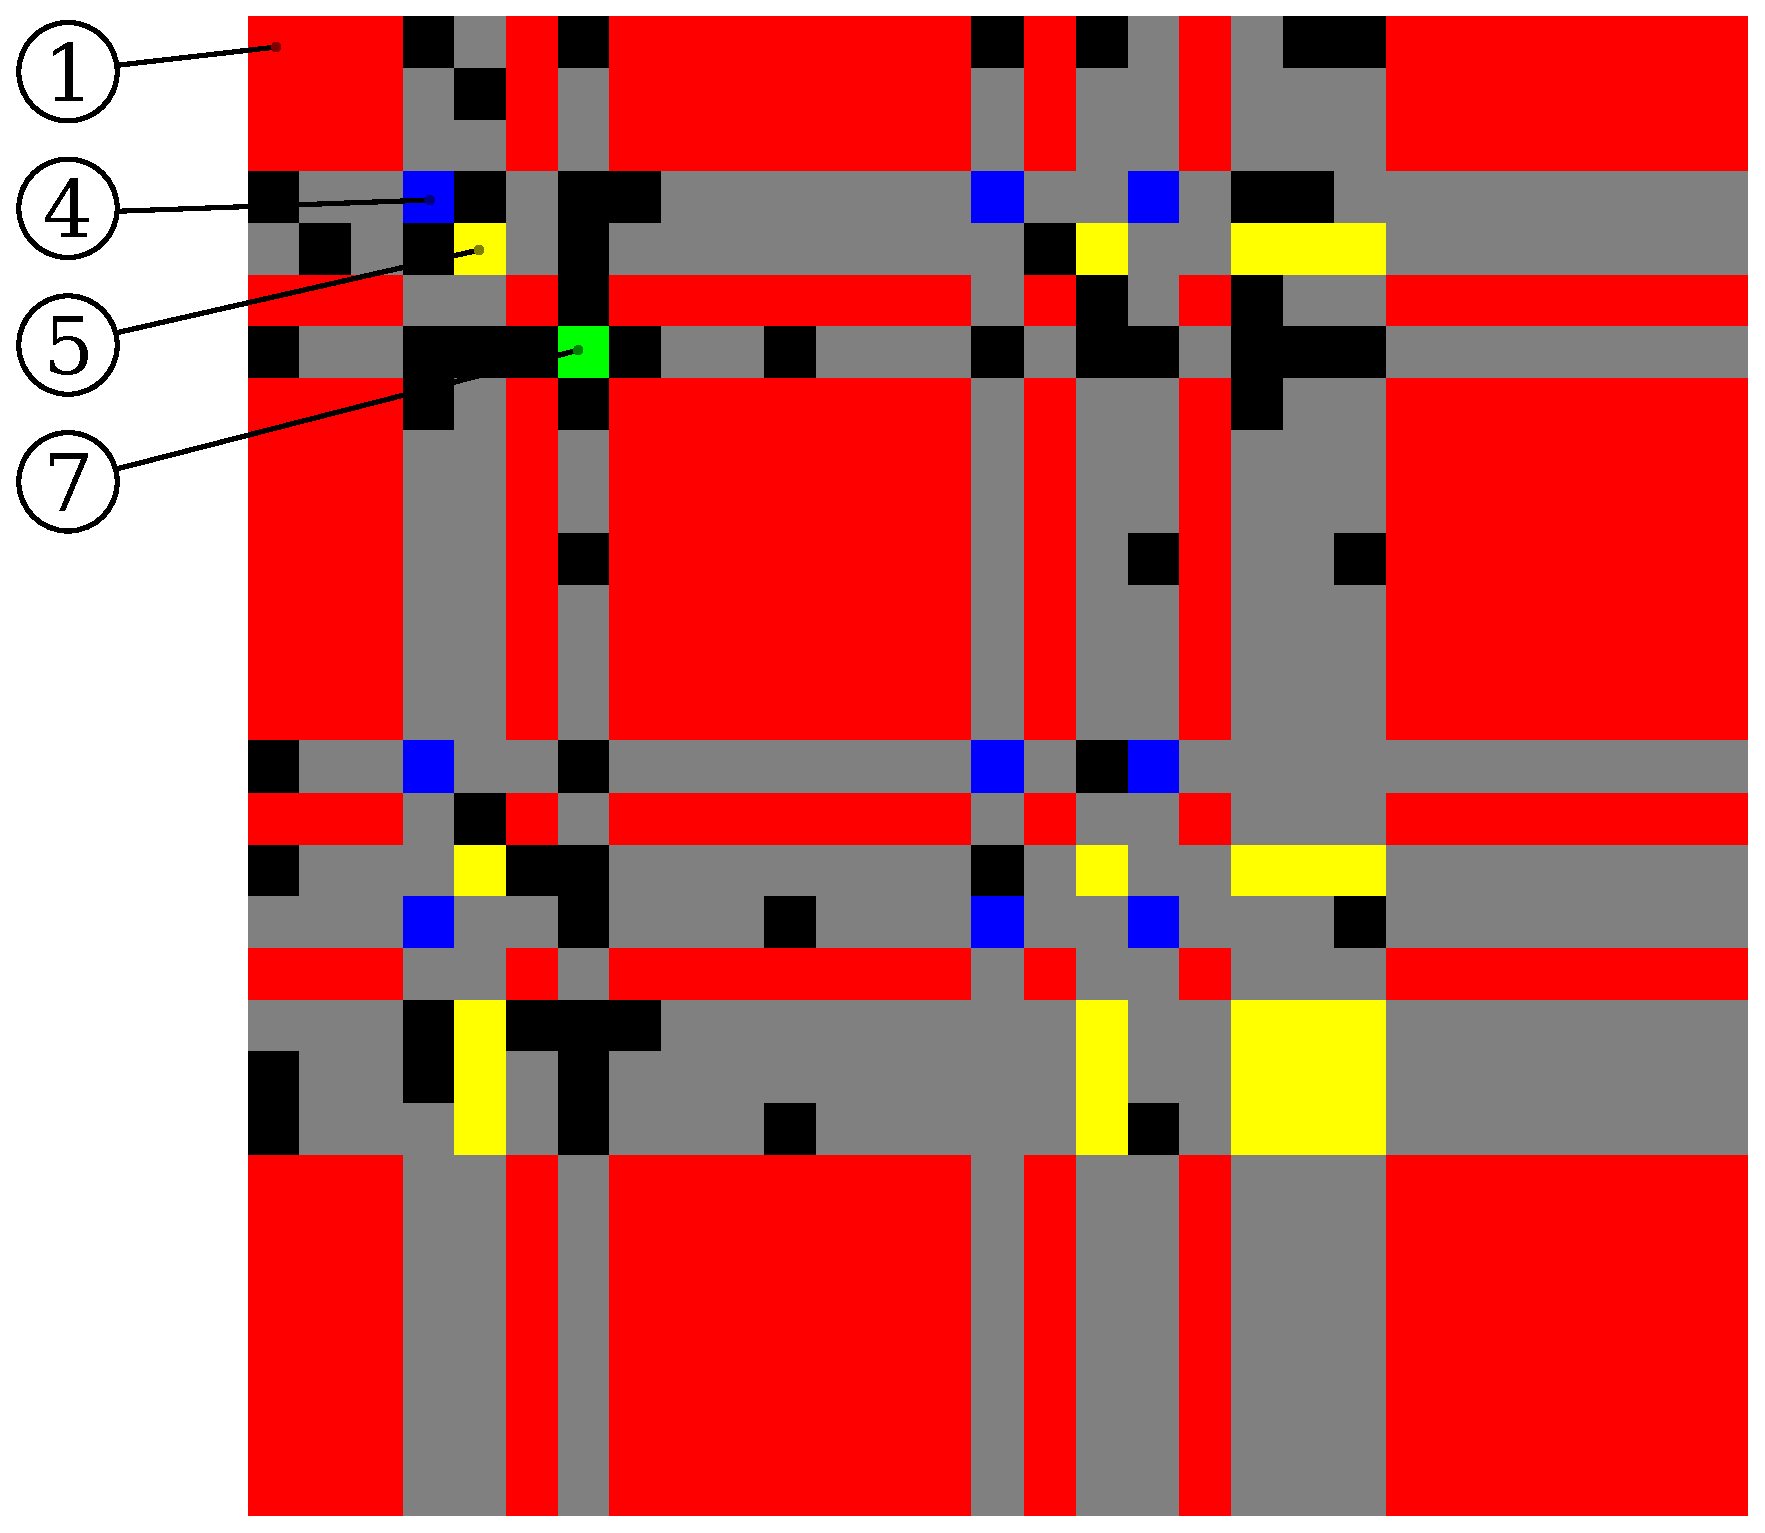
\includegraphics[height=\bfigh]{media/random_cliques}}
\qquad
\subfigure[Reduced Representation]{
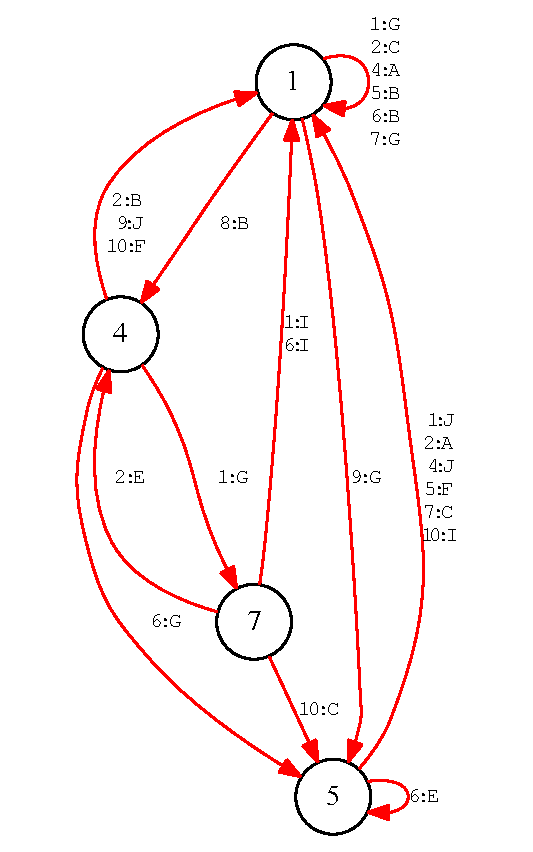
\includegraphics[height=\bfigh]{media/random_alg-2}}
\caption{\emph{Greedy Reduction Algorithm} A ``running clique'' is kept, to which new states are added until all remaining states are
incompatible with at least one state in the clique.  Then, a new clique is begun.  
Here, the cliques are 
$\{1, 2, 3, 6, 8, 9, 10, 11, 12, 13, 14, 16, 19, 22, 26, 27, 28, 29, 30, 31, 32\}$ (red),
$\{4, 15, 18\}$ (blue), $\{5, 17, 21, 22, 23\}$ (yellow), and $\{7\}$ (green). (d) shows the resulting policy graph once 
}
\end{figure}
For practical computation of reducibility, we'll start with the weaker condition of compatibility.

\subsection{Reducibility Relations}

\begin{definition}[Reducibility]
For a given policy $P=\ang{\C,\U,\T,\Y}$, two contexts $c_1, c_2\in\C$ are \textbf{reducible} (write $c_1\sim c_2$) if there exists a representation 
$\ang{\R,\S}$ of $P$ such that $\R(c_1)=\R(c_2)$.  Likewise, for a given representation $R=\ang{\R,\S}$, two states 
$s_1,s_2\in\S$ are \textbf{reducible} if there exists a reduction $(\phi, \ang{\R\1,\S\1})$ of $R$ such that
$\phi(s_1)=\phi(s_2)$.
\end{definition}
Observe that for any representation $\ang{\C,\R,\U,\S,\T,\Y}$,
the contexts $c_1, c_2\in\C$ are reducible if and only if the states $\R(c_1)$ and $\R(c_2)$ are reducible.
Observe also that for incompletely-determined policies, reducibility is a symmetric but not-necessarily-transitive relation
\begin{example}[Non-Transitive Reducibility]
Suppose $\Y=\{1,2,3\}$, $\C=\{\emptyset, (1), (2), (1,3), (2,3)\}$, \mbox{$\U=\{A,B\}$}, and 
\begin{equation}
\T(c) = \begin{cases}
A&c\in\{(1), (1,3)\}\\
B&c\in\{(2), (2,3)\}
\end{cases}.
\end{equation} 
Observe that, under this policy, $\emptyset\sim(1)$ and $\emptyset\sim(2)$, but $(1)\not\sim(2)$, 
since $\T(1,3)\neq\T(2,3)$.
\end{example}
However, it can be shown that, under a completely-determined policy, reducibility induces an equivalence relation.  
In either case, we compute reducibility using the following criterion:
\begin{lemma}
Two contexts $c_1,c_2\in\C$ are reducible iff 
\begin{equation}
\T(c_1,s)=\T(c_2,s)\qtx{for all}s\in\Y^*\qtx{such that}(c_1,s),(c_2,s)\in\C
\end{equation} 
\end{lemma}

This informs the following algorithm
\begin{algorithm}                      % enter the algorithm environment
\label{algo: Hopcroft}
\caption{(Hopcroft) Compute Reducibility Relations}          % give the algorithm a caption
\label{alg1}                           % and a label for \ref{} commands later in the document
\begin{algorithmic}                    % enter the algorithmic environment
  \REQUIRE A representation $\ang{\C,\R,\U,\S,\T,\Y}$
  \ENSURE A reducibility matrix $A:\S\times\S\to\{\TRUE,\FALSE\}$.
  \bigskip
  
  \STATE $A(s_1, s_2)\Leftarrow \TRUE$\quad for all $s_1,s_2\in\S$.
  \REPEAT
    \STATE $isChanged \Leftarrow \FALSE$
    \FOR{$s_1<s_2\in \S$}
	  
	  \IF{$A(s_1,s_2)=\TRUE$}
		\FOR{$c_1\in\R\inv(s_1),\,c_2\in\R\inv(s_2)$}
		  \FOR{$y\in\Y_{c_1}\cap\Y_{c_2}$}
			\IF{$\T(c_1,y)\neq\T(c_2,y)\;\;\text{or}\;\;^{\sim}A(\R(c_1,y),\R(c_2,y))$}
			  \STATE $A(s_1,s_2)\Leftarrow\FALSE$.
			  \STATE $isChanged\Leftarrow\TRUE$.
			\ENDIF
		  \ENDFOR
		\ENDFOR
	  \ENDIF
    \ENDFOR
  \UNTIL{$^{\sim}isChanged$} 
\end{algorithmic}
\end{algorithm}

\subsection{Bit-at-a-Time}
The Bit-at-a-Time reduction, proposed by Andrea Censi, generates a set of states one at a time,
separating ambiguous contexts recursively.  An ambiguous context is an (input, state) pair for
which more than one output is defined.  Ambiguities which arise in shorter sequences are separated first.
This results in an FSM whose graph structure is a subtree of the original decision tree.
\begin{figure}
\centering
\subfigure[Decision Tree]{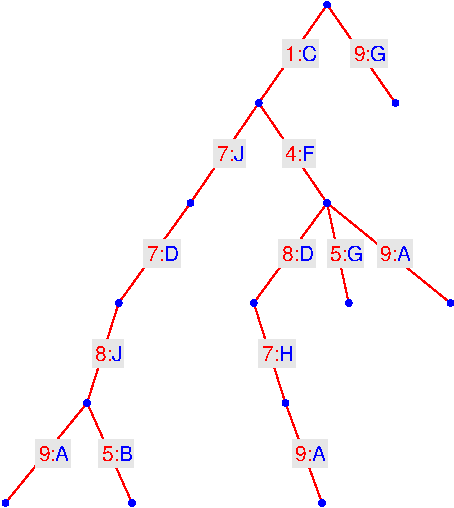
\includegraphics[height=2in]{cdiag1}}
\subfigure[Partitioned Tree]{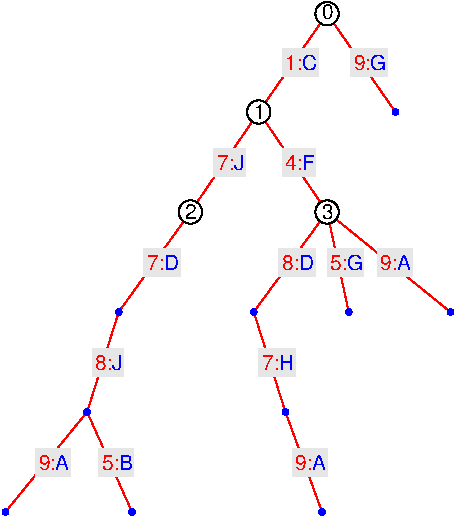
\includegraphics[height=2in]{cdiag2}}
\subfigure[Reduced FSM]{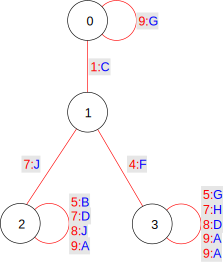
\includegraphics[width=1in]{cdiag3}}
\caption{\emph{Censi's Bit-at-a-time Algorithm}}
\end{figure}
 
\subsection{Greedy Covering}

Although reducibility is not an equivalence relation, 
any reduction $\phi:\S\to\S\1$ induces an equivalence relation,
partitioning $\S$ into cliques of mutually-reducible states, i.e.
\begin{equation}
\S = \bigsqcup_{s\1\in\S\1}\phi\inv(s\1),\qtx{where}\phi(s_1)=\phi(s_2)\implies A(s_1,s_2)
\end{equation}
Thus, a minimum 
reduction
induces a minimum clique partition of the
reducible states of a representation.
\subsection{Assembling Cliques}
\begin{notation}[Arrow notation]
For a policy $P=\ang{\C,\U,\T,\Y}$, 
write $c\to c\1$ if $c=(c_1,\ldots,c_i)\in\C_i\subseteq\C$ and 
$c\1=(c_1,\ldots,c_i,y)\in\C_{i+1}\subseteq\C$, for some $i$.  For a representation $\ang{\R,\S}$ of $P$,
write $s_1\to s_2$ if there are $c_1\in f\inv(s_1)$ and $c_2\in f\inv(s_2)$ such that $c_1\to c_2$.
\end{notation}
We propose the following, greedy, approximate algorithm
\begin{algorithm}                      % enter the algorithm environment
\caption{Greedy Clique Covering}          % give the algorithm a caption
\label{alg2}                           % and a label for \ref{} commands later in the document
\begin{algorithmic}                    % enter the algorithmic environment]
  \REQUIRE A representation $\ang{\C,\R,\U,\S,\T,\Y}$ with $s_1<s_2$ only if $s_2\not\to s_1$.
  \REQUIRE A reducibility matrix $A:\S\times\S\to\{\TRUE,\FALSE\}$ as computed by Algorithm \ref{alg1}.
  \ENSURE A partition function $\phi:\S\to\S\1$ with $\phi(s_1)=\phi(s_2)$ only if $A(s_1,s_2)$.
  \bigskip
  
  \STATE $\S\1\Leftarrow\S$
  \STATE $\phi\Leftarrow id_{\S}$
  \STATE $unused\Leftarrow\S$
  \WHILE{$|unused|>0$}
	\STATE $s_1\Leftarrow\min(unused)$
	\STATE $unused\Leftarrow unused\andn\{s_1\}$
	\FOR{$s_2\in unused$}
	  \IF{$A(s_1,s_2)$}
		\STATE $\phi(s_2)\Leftarrow s_1$
		\STATE $unused\Leftarrow unused\andn\{s_2\}$
	  \ENDIF
	\ENDFOR
  \ENDWHILE
\end{algorithmic}
\end{algorithm}
In order find the absolute minimum representation of a
given policy, it suffices to run the greedy algorithm on all
possible orderings of its states: 
Given a minimum clique covering 
$S=\{s_{c_{11}}, s_{c_{12}}, \ldots, s_{c_{1 N_1}}\}$
$\cup$
$\{s_{c_{21}}, s_{c_{22}}, \ldots, s_{c_{2 N_2}}\}$
$\cup$ $\cdots$ $\cup$
$\{s_{c_{K1}}, s_{c_{K2}}, \ldots, s_{c_{K N_K}}\}$,
feed states to the greedy algorithm in the order in which they are written.
%i.e. add from the list $s_{c_{11}}, s_{c_{12}}, \ldots, s_{c_{1N_1}}, s_{c_{21}},\ldots$ until
Failure to add states to a running clique will occur only once per clique in the minimal covering (exactly $K$ times)
\footnote{If more than $K$ times, then some running clique },
so the greedy algorithm will produce a minimum covering.  Of course, 
exhaustively checking every ordering will end up taking exponential time.
In fact, it has been shown that the minimum clique cover problem is NP-hard \cite{karp72}.
\subsection{Maximal Anticlique}
Alberto and Sim\~ao \cite{4813796} propose a heuristic to 
increase the likelihood that a greedy algorithm produces a minimum clique covering --
First, a maximum anticlique is found in the compatibility graph (This is also an NP-hard problem \cite{karp72},
but the size of the maximum anticlique generally grows more slowly than the graph itself).
Now, each state in the maximum anticlique must belong to a different clique in the minimum
clique covering.  Also, every remaining state must be compatible with at least one of the states in the 
anticlique (or else violate the maximality of the anticlique).  The greedy algorithm then proceeds,
taking first the states in the maximum anticlique, then the remaining states
It can easily be shown that an ordering of this type will produce a 
minimum reduction.  The number of such orderings still grows exponentially with 
the number of states, but in practice it grows significantly more slowly.
\begin{figure}
\setcounter{subfigure}{0}
\centering
\subfigure[Bad Ordering]{
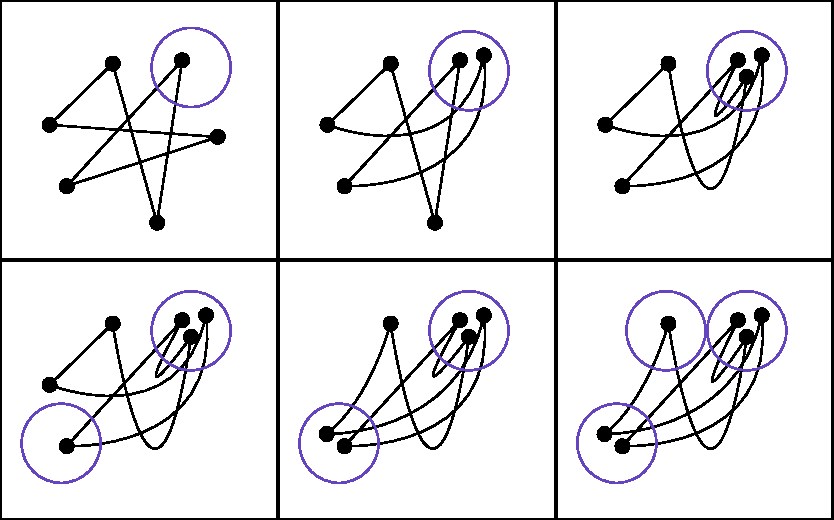
\includegraphics[width=4in]{bad_greedy.pdf}}
\subfigure[Good Ordering]{
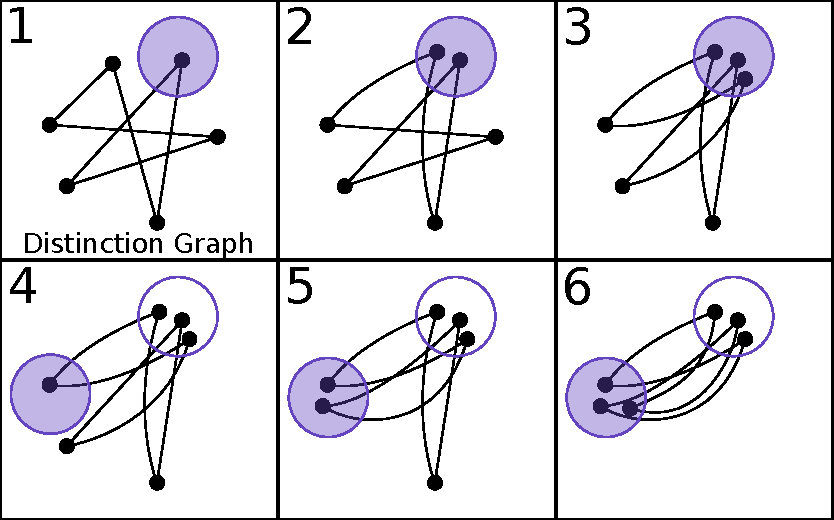
\includegraphics[width=4in]{good_greedy.pdf}}
\caption{\emph{Greedy Algorithm on Pathological Trees}
\label{goodbad_order}
Here we illustrate the dependence of greedy algorithms
on the order of their inputs.
In the first set of figures (a), we proceed randomly,
greedily adding random states to a running clique until none can be added
(no two states sharing an edge in the distinction graph can be part of the same clique).
This results in one more clique than is necessary - 
proceeding counterclockwise, we cover the set with only two cliques.
Alberto and Sim\~ao's
maximum anticlique algorithm
fares no better, as the maximal anticlique has size 2.
}
\end{figure}

\subsection{Comparisons}
Two types of random FSMs were generated to test the correctness and numerical efficiency of the 
algorithms described above.
\subsubsection{Poisson Random Tree}
A Poisson random tree is an decision policy generated by recursively adding
      $X\sim\operatorname{Poisson(\lambda)}$ children to each new node of 
      an existing policy.
      We conditioned this result on the outcome that the  process not terminate before the tree 
      reaches depth $H$ (contains a sequence of length $H$ or greater).
      These decision policies are well-studied in decision theory, as they model birth/death processes where
      individuals continuously produce
      offspring at a rate of $\lambda$ per lifetime.
\begin{figure}
\centering
\subfigure[Poisson Tree Growth Trend]{
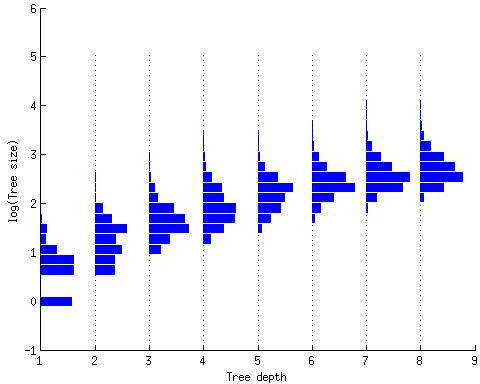
\includegraphics[height=1.8in]{poiss_size.jpg}\qquad
}
\subfigure[Tree, Depth 10]{
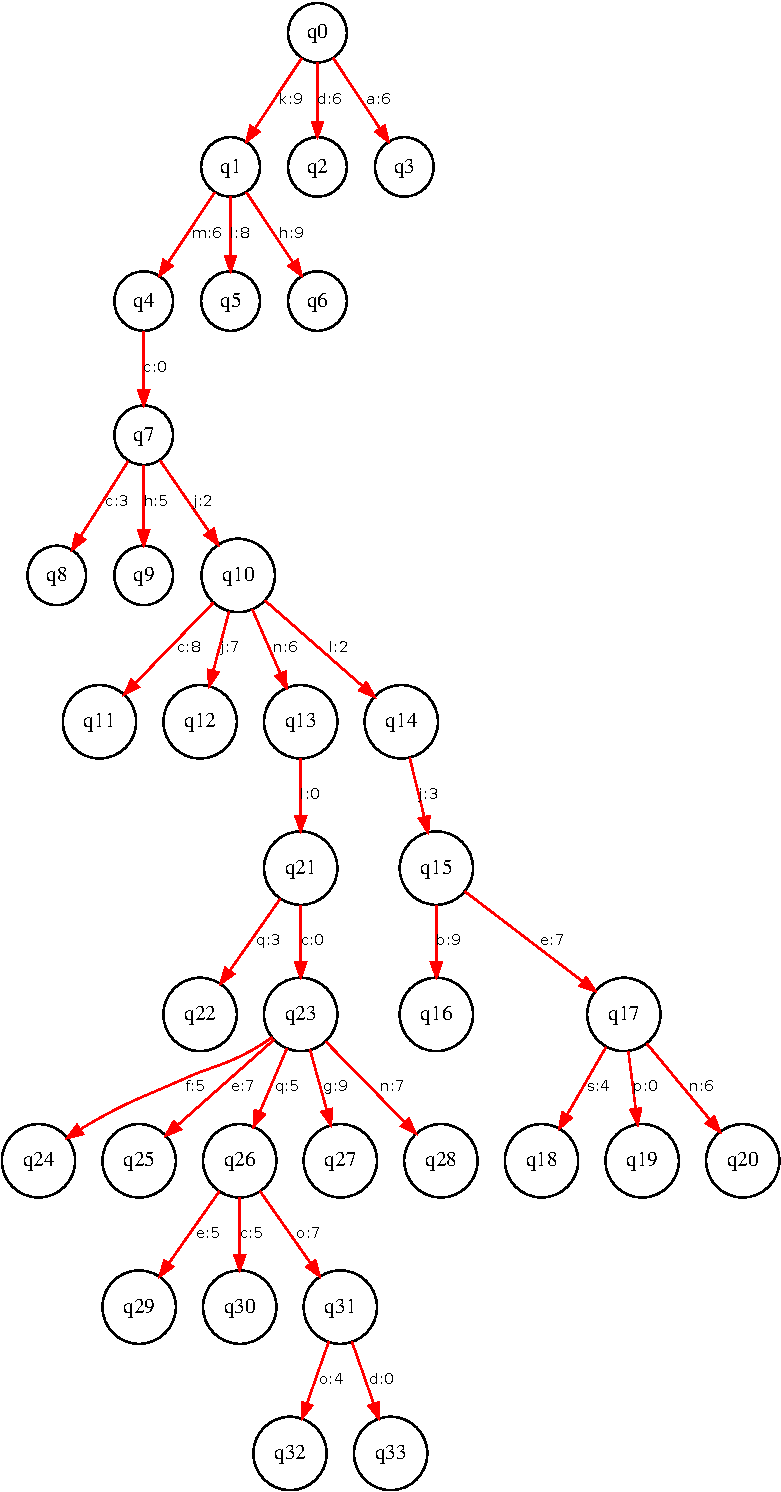
\includegraphics[height=1.8in]{big_tree_left.pdf}}
\caption{\emph{Poisson Random Tree}}
\end{figure}
\subsubsection{Pathological Tree}
The ``pathological'' tree is a policy of depth 2 with $6n+1$ contexts.
was designed to frustrate the algorithm of Alberto and Sim\~ao.
Each of its states at depth 1 is incompatible with exactly two others.  
The resulting distinction graph consists of disjoint rings. 
The order in which states are added to cliques is critical.  
Half of all orderings result in a three-state FSM, whereas the minimum number of states is two.
\begin{figure}
\centering
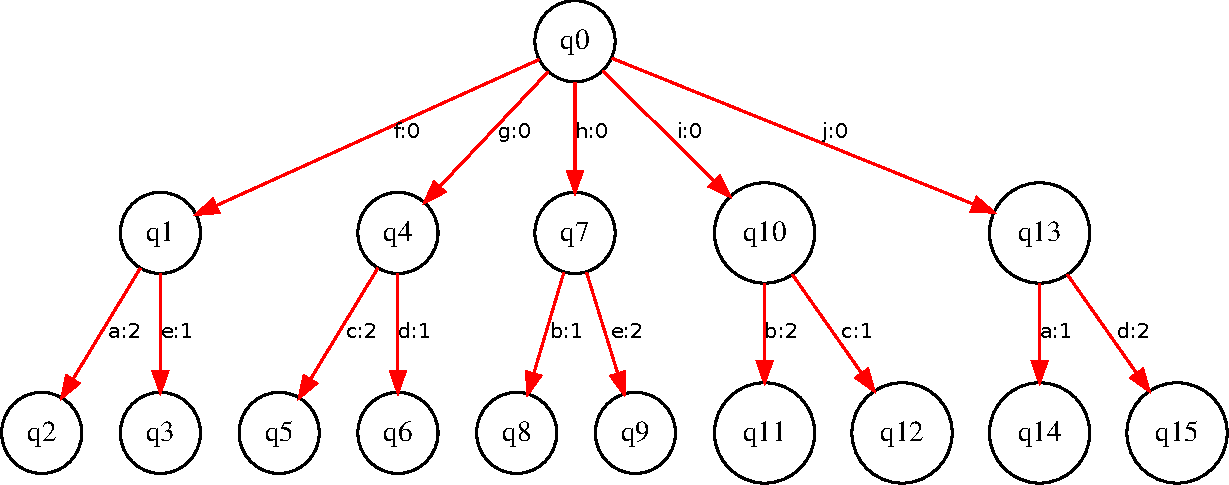
\includegraphics[width=4in]{big_patho_tree.pdf} 
\caption{\emph{Pathological Tree} }
\end{figure}
\begin{figure}
\centering
\subfigure[\scriptsize{Original}]{
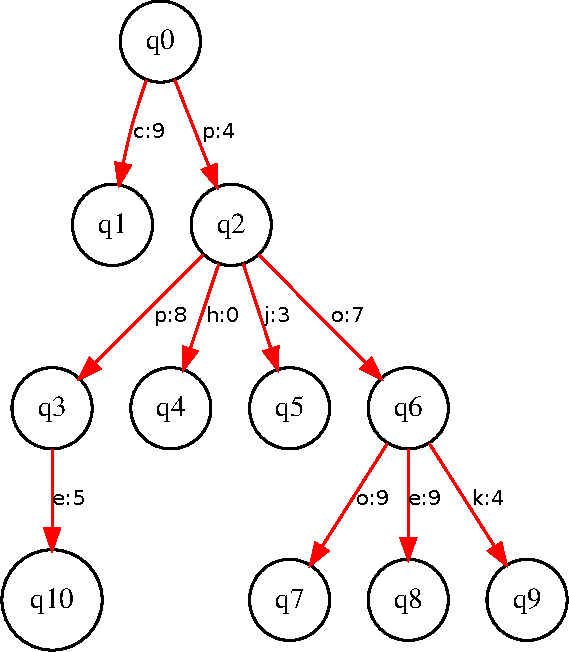
\includegraphics[scale=0.25]{orig.pdf}
}
\subfigure[\scriptsize{Bit-at-a-Time}]{
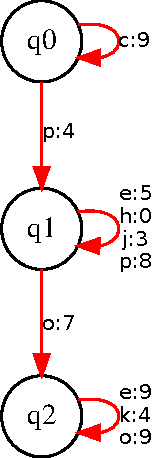
\includegraphics[scale=0.3, angle=35]{censi.pdf}
}
\subfigure[\scriptsize{Greedy}]{
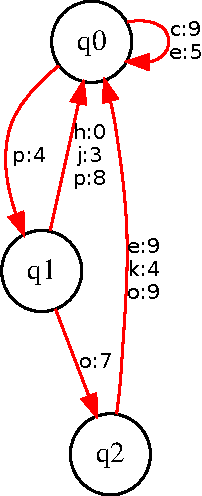
\includegraphics[scale=0.3, angle=35]{josh.pdf}
}
\subfigure[\scriptsize{Alberto-Sim\~ao}]{
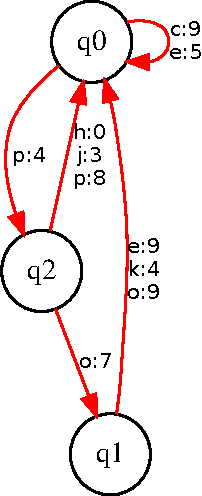
\includegraphics[scale=0.3, angle=35]{alberto.pdf}
}
\subfigure[\scriptsize{Exact}]{
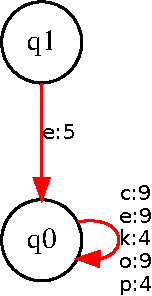
\includegraphics[scale=0.3, angle=35]{exact.pdf}
}
\caption{\emph{Typical Reductions}
Here we contrast the results of the various reduction algorithms introduced above.
The Bit-at-a-Time method (b) produces a minimal sub-tree of
the canonical policy.
The last three methods are equivalent up to a reordering of states,
so reductions (c) and (d) are practically identical. 
}
\end{figure}
\subsection{Discussion}
The Bit-at-a-time algorithm consistently underperformed all of the greedy clique-assembly
algorithms, both in time requirements (finding the earliest ambiguous
contexts took $O(N^3)$ time), and in reduction performance.  However, the 
subtree property of its output may make it better suited for applications
that require running ``in-place''.

Greedy algorithms seem to be the best choice, although they left something to be desired.
Although better heuristics helped to reduce the likelihood of non-optimal reduction,
it was not hard to find policies that could trip them up.

Although it is not certain how much of this work can be generalized to more
interesting robotics applications (e.g. continuous time, continuous input/output,
probabilistic systems), our results suggest that some general-purpose
ambiguity-splitting scheme could eventually be applied to all types of POMDP solvers.
\begin{figure}
\centering
\subfigure[Poisson Trees Reduced vs.\ Orig.\ Size]{
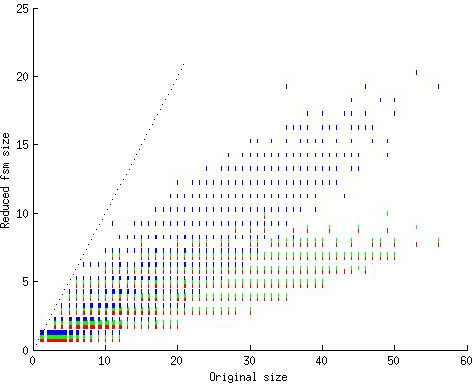
\includegraphics[height=1.7in]{poiss_orig.jpg}}\qquad
\subfigure[Patho.\ Trees Reduced vs.\ Orig.\ Size]{
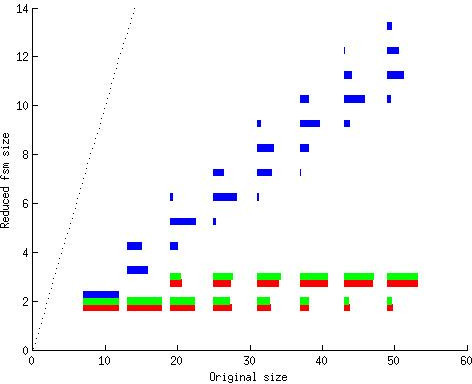
\includegraphics[height=1.7in]{patho_orig.jpg}}\\
\subfigure[Poisson Trees Reduced vs.\ Min.\ Size]{
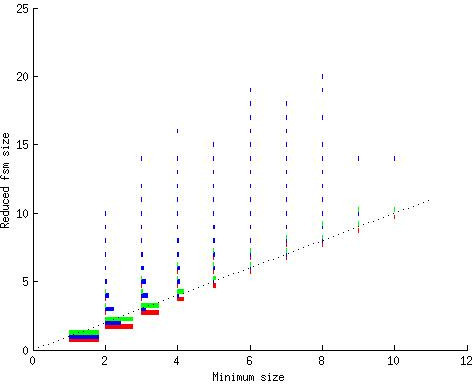
\includegraphics[height=1.7in]{poiss_exact.jpg}}\qquad
\subfigure[Patho.\ Trees Reduced vs.\ Min.\ Size]{
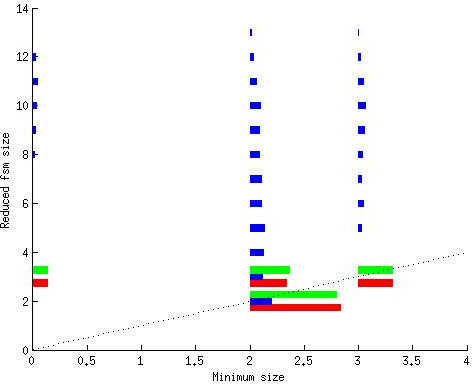
\includegraphics[height=1.7in]{patho_exact.jpg}}\\
\subfigure[Algo.\ Runtimes on Poison Trees]{
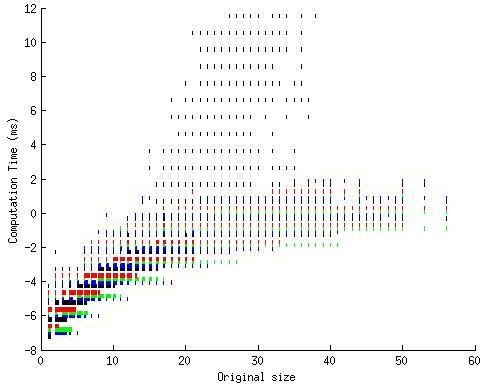
\includegraphics[height=1.7in]{poiss_time.jpg}}\qquad
\subfigure[Algo.\ Runtimes on Patho.\ Trees]{
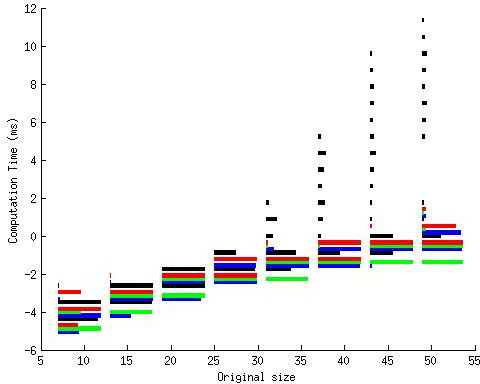
\includegraphics[height=1.7in]{patho_time.jpg}}
\caption{\emph{} {Red} bars pertain to Alberto and Sim\~ao's method, 
{blue} bars pertain to the bit-at-a time method, 
{green} bars pertain to the greedy clique completion method, 
and
{black} bars pertain to an exhaustive search for a minimal reduction.
The black dotted line in the first two rows of figures plots the line $y=x$.  Note the greater
proportion (50\% or greater) of nonoptimal reductions in th
pathological (``Patho.'') examples, and the clear separation in performance between 
the bit-at-a-time and greedy methods.
}
\end{figure}